\subsubsection{Information}
\begin{itemize}
	\item \textbf{Course Name:} \href{https://www.coursera.org/learn/high-fidelity-designs-prototype}{Create High-Fidelity Designs and Prototypes in Figma}
	\item \textbf{Instructor:} \href{https://www.coursera.org/instructor/google-career-certificates}{Google Career Certificates}
	\item \textbf{Level:} Beginner
	\item \textbf{Enrolled on:} June 8, 2024
	\item \textbf{Finished on:} July 6, 2024
	\item \textbf{Grade Achieved:} 89.86\%
\end{itemize}

\subsubsection{Certificate}
\begin{flushleft}
	\begin{figure}[!ht]
		\centering
		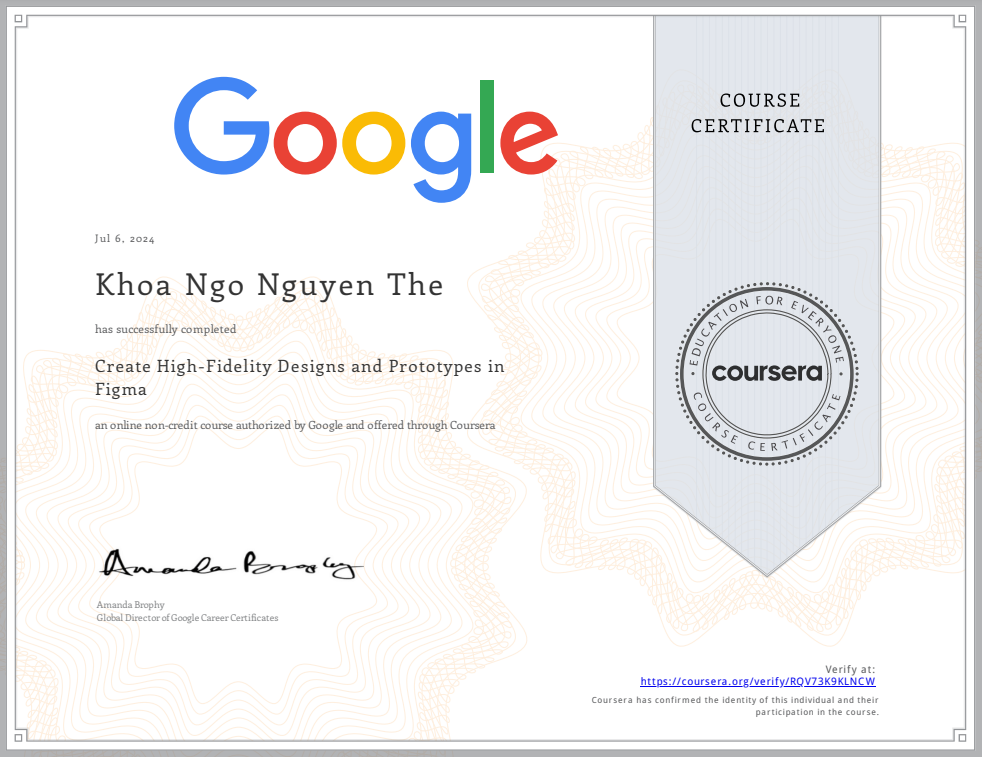
\includegraphics[width=0.85\textwidth]{imgs/Course5.png}
		\caption{Course 5 Certificate}
	\end{figure}

	Visit the online certificate for more info \href{https://www.coursera.org/account/accomplishments/verify/RQV73K9KLNCW}{here}
\end{flushleft}

\subsubsection{Summary}
\begin{flushleft}
	What I have learned after completing this course:
	\begin{itemize}
		\item Build mockups and high-fidelity prototypes in the design tool Figma.
		\item Define and apply common visual design elements and principles.
		\item Demonstrate how design systems can be used to organize, standardize, and enhance designs.
		\item Understand the role of design critique sessions and feedback while iterating on designs.
	\end{itemize}
\end{flushleft}

\subsubsection{Details}
\begin{flushleft}
	\begin{description}
		\item[Module 1:] Starting to create mockups
		      \begin{itemize}
			      \item I have used visual design elements, like typography, color, and iconography to create mockups.
			      \item I have applied visual design learnings to build on the mobile app designs I've been working on throughout the certificate program.
		      \end{itemize}
		\item[Module 2:] Applying visual design principles to mockups
		      \begin{itemize}
			      \item I have used visual design principles to refine mockups and emphasis to guide users to the most important parts of a page.
			      \item I have applied hierarchy, scale, and proportion to organize the elements on each page of my app.
			      \item I have revisited Gestalt Principles, like similarity, proximity, and common region, to help users interpret my designs easily.
		      \end{itemize}
		\item[Module 3:] Exploring design systems
		      \begin{itemize}
			      \item I have known the parts of a design system, as well as the benefits of using a design system.
			      \item I have examined various companies' design systems, and had an opportunity to use them in my own mockups.
			      \item I have also learnt how to use and create sticker sheets in Figma.
		      \end{itemize}
		\item[Module 4:] Creating high-fidelity prototypes
		      \begin{itemize}
			      \item I have turned my mockups into a prototype that's ready for testing.
			      \item I have explored two new concepts, gestures and motion, which can help enrich the user experience and increase the usability of prototypes.
		      \end{itemize}
		\item[Module 5:] Testing and iterating on designs
		      \begin{itemize}
			      \item I have conducted a usability study to test my high-fidelity prototype of a mobile app and learnt how to hand off designs to engineers for production.
			      \item I have analyzed the feedback I received to come up with actionable insights and iterate on my designs.
			      \item I have turned everything I learnt about user research, ideation, wireframes, designs, and prototypes into a case study for my professional UX portfolio.
		      \end{itemize}
	\end{description}
\end{flushleft}